\documentclass[11pt]{article}
\usepackage[a4paper,margin=25mm]{geometry}
\usepackage[T1]{fontenc}
\usepackage{lmodern,microtype,amsmath,amssymb,amsthm,booktabs,array,tikz}
\usepackage{enumitem,xurl}
\usepackage[hidelinks]{hyperref}
\usepackage{fancyhdr}
\pagestyle{fancy}\fancyhf{}
\fancyhead[L]{\small Parity and constructive triangle-tiling spectra}
\fancyhead[R]{\small Research note}
\fancyfoot[C]{\thepage}
\setlength{\headheight}{15pt}
\setlength{\parskip}{4pt}
\setlength{\parindent}{0pt}
\newtheorem{theorem}{Theorem}
\newtheorem{lemma}[theorem]{Lemma}
\newtheorem{corollary}[theorem]{Corollary}
\newcommand{\Z}{\mathbb Z}
\newcommand{\NN}{\mathbb Z_{\ge0}}
\title{Parity and constructive spectra\newline for congruent triangle tilings}
\author{Denis Paliy\thanks{Research conducted with assistance from ChatGPT. The mathematical arguments and exact computations are internal to this project, not external referee reports or a proof-assistant formalization.}}
\date{30 September 2026}
\begin{document}
\maketitle
\begin{abstract}
Two signed-direction boundary values have the same parity as the number of tiles. Their half-sum forces the side of an equilateral target to be divisible by $ab$ for a primitive rational tile with a $60^\circ$ or $120^\circ$ angle opposite $c$. Half-differences give short proofs of the previously recorded isosceles and F1 necessary spectra. An exact coin-representation calculation refines a trapezoidal construction and supplies every equilateral multiplier above $3(\lfloor A/B\rfloor+2)$ or $3(\lfloor A/B\rfloor+1)$, respectively, where $A=\max(a,b)$ and $B=\min(a,b)$. An exact construction for $(45,32,67)$ at multiplier $9$ lies below the cutoff $12$ in the literal formulation of Zhang's Conjecture 2 in the inspected version 4. These results do not classify the small multipliers and do not solve Erd\H{o}s problem 634 in full.
\end{abstract}

\section{Scope and prior work}
All dissections are finite and permit reflections and arbitrary T-junctions. A tile merely touching an external side at a vertex need not have an edge there. In the cancellation argument below, subdivision at all T-junctions is performed explicitly.

The direction-functional framework comes from the existing literature and source corpus. In particular, Bonfioli's manuscript~\cite{Bonfioli}, theorem labelled \texttt{thm:spectrum}, already gives the isosceles and F1 necessary forms in Section~\ref{sec:ratios}. We give a shorter derivation rather than claiming those forms as new. The constructive building blocks are Zhang's three-triangle trapezoids and strip parallelograms~\cite{Zhang}. Our refinement uses the exact residues of the base lengths needed by that construction. No priority claim is made.

Theorems here assume a primitive integer tile. The wider relevance of that hypothesis is supported by the rationality theorem of Beeson and Zhang~\cite{Rationality}; it is not an extra input to the proofs once the fixed-tile assumptions are imposed. Neither the previous $N=105$ certificates nor the candidate prime-count proof is used.

\section{Two characters and parity}
Let the tile have sides $a,b,c$ opposite $\alpha,\beta,\gamma$, where $\gamma$ is $\pi/3$ or $2\pi/3$, and $\alpha/\pi$ is irrational. Normalize a target side to be horizontal. All directed tile edges have directions in
\[
G=\{n\alpha+j\pi/3\pmod{2\pi}:n\in\Z,\ j\in\Z/6\Z\}.
\]
Indeed, the adjacency graph of tiles sharing a positive-length segment is connected: a path through the interior avoiding the finitely many vertices proves this. Crossing an adjacency changes directions by integer combinations of tile angles. Irrationality makes the displayed representation unique.

Define
\[
f(n\alpha+j\pi/3)=(-1)^j,\qquad
g(n\alpha+j\pi/3)=(-1)^{n+j}.
\]
Both functions change sign when a directed edge is reversed. Let $F_f(P)$ be the sum of edge length times $f$ around a counterclockwise polygonal boundary, and define $F_g$ similarly. At a T-junction, subdivide the longer edge. The contributions of all internal subsegments cancel, so the values add under dissection.

Each rotated or reflected congruent tile contributes either sign of the reference tile's value. For a reflection, reverse traversal to restore counterclockwise orientation; this changes the sign while negating directions, which does not change the character. Consequently a tiling by $N$ pieces gives normalized values
\begin{equation}
 U,V\in\Z,\qquad U\equiv V\equiv N\pmod2. \label{eq:parity}
\end{equation}
In particular, both their half-sum and their half-difference are integers.

Traverse a reference tile with the $c$-edge in direction zero. For $\gamma=2\pi/3$, the $a,b$ directions are $\alpha+2\pi/3,\alpha+\pi$, so its values are
\begin{equation}
 X=c+a-b,\quad Y=c+b-a,\quad XY=3ab. \label{eq:120}
\end{equation}
For $\gamma=\pi/3$, the $a,b$ directions are $\alpha+\pi/3,\alpha+\pi$, giving values $-A_0,B_0$, where
\begin{equation}
 A_0=a+b-c,\quad B_0=a+b+c,\quad A_0B_0=3ab. \label{eq:60}
\end{equation}
These follow from $c^2=a^2\pm ab+b^2$. Primitivity implies pairwise coprimality: a prime dividing any two sides divides the third by the norm equation.

\section{Equilateral scale divisibility}
\begin{theorem}\label{thm:equilateral}
For a primitive integer tile as above, any tiled equilateral target of side $S$ satisfies
\[
\boxed{S=abm,\qquad N=abm^2,\qquad m\in\Z_{>0}.}
\]
\end{theorem}
\begin{proof}
A target side is a concatenation of whole integer-length edges, so $S$ is an integer. The three target directions are $0,2\pi/3,4\pi/3$; both boundary values are $3S$.

In the $120^\circ$ case, $U=3S/X$, $V=3S/Y$, and
\[
\frac{U+V}{2}=\frac{3S(X+Y)}{2XY}=\frac{Sc}{ab}\in\Z.
\]
Since $\gcd(c,ab)=1$, this forces $ab\mid S$.

In the $60^\circ$ case set $u=-U=3S/A_0$ and $v=V=3S/B_0$. Negating $U$ does not change its parity. Thus
\[
\frac{u+v}{2}=\frac{S(a+b)}{ab}\in\Z.
\]
Now $\gcd(a+b,ab)=1$ gives the same divisibility. The area ratio is $N=S^2/(ab)$ in either case.
\end{proof}

Conversely, $S=abm$ passes both of these arithmetic tests. Their values become $mY,mX$ or $-mB_0,mA_0$, respectively. Modulo two, the norm equation gives
\[
c\equiv a+b+ab\pmod2,
\]
so these values have the parity of $abm^2$. Hence Theorem~\ref{thm:equilateral} describes the \emph{invariant-admissible} spectrum exactly; this converse is not a geometric existence theorem.

This proves the divisibility assertion of Conjecture 1 of the inspected Zhang v4 and the divisibility component of its $60^\circ$ extension. It does not prove the conjectured sharp cutoff.

For instance, for $(a,b,c)=(5,16,19)$ one has $X=8,Y=30$. Integrality alone allows $S=40h$. Then $U=15h$, $V=4h$, so their equal parity forces $h$ even. Thus $80\mid S$. No squarefree-side assumption was used.

\section{Half-differences for two ratio families}\label{sec:ratios}
Assume now $c^2=a^2+ab+b^2$. The F1 target has primitive side proportions $(a,c,a+b)$, and the isosceles target with base angle $\alpha$ has proportions $(c,c,a+2b)$. Their scales $\lambda$ are integers, by whole external edge lengths and B\'ezout.

For the isosceles proportions, note that $\gcd(c,a+2b)=1$. A common prime would divide $3b^2$, whereas $3\nmid c$: if $3\mid c$, then $a\equiv b\pmod3$ and $c^2\equiv3b^2\pmod9$, contradicting primitivity.

For F1, the directed sides have directions $0,2\pi/3,\pi+\alpha$. The values are
\[
 U=\frac{\lambda(2a+b-c)}X=\frac{\lambda(c-a)}b,
 \qquad
 V=\frac{\lambda(2a+b+c)}Y=\frac{\lambda(c+a)}b.
\]
Therefore
\[
\frac{V-U}{2}=\frac{\lambda a}{b}\in\Z.
\]
Coprimality gives $b\mid\lambda$, and the area equation yields
\begin{equation}
N=b(a+b)m^2.\label{eq:f1}
\end{equation}
For the isosceles target, the directed sides have directions $0,\pi-\alpha,\pi+\alpha$. This gives
\[
 U=\frac{\lambda(c-a-b)}b,\qquad
 V=\frac{\lambda(c+a+b)}b,
 \qquad \frac{V-U}{2}=\frac{\lambda(a+b)}b\in\Z.
\]
Again $b\mid\lambda$, and
\begin{equation}
N=b(a+2b)m^2.\label{eq:iso}
\end{equation}
All identities are obtained by multiplying out and substituting the norm equation. Conversely $\lambda=bm$ satisfies both parity tests. This recovers the previously recorded spectra~\cite{Bonfioli} without prime-adic case analysis. Small members of these forms need not be geometrically realizable.

\section{An exact residue calculation for the construction}
Relabel $a,b$ for this section so that $a>b>1$, and write
\[
a=qb+r,\qquad q\ge1,\quad1\le r<b,\quad L=ab.
\]
An ideal trapezoid here has shorter base $x$, legs $h$, longer base $x+h$, and acute angles $60^\circ$.

For $120^\circ$ tiles, the basic trapezoid has shorter base $K=a^2+b^2$, legs $L$, and longer base $c^2$. It consists of three integer-scale copies of the original tile, at scales $a,b,c$. For $60^\circ$ tiles, $K=c^2=a^2+b^2-L$, with the same three scales. Explicit coordinates are supplied below; these are the basic constructions of~\cite{Zhang}.

A parallelogram with angles $60^\circ,120^\circ$ and sides $L$ and $R=ax+by$, $x,y\in\NN$, is tileable. Split the $R$ direction into $x$ strips of width $a$ and $y$ of width $b$; divide the $L$ direction respectively into $b$-steps or $a$-steps. Each cell divides into two original tiles. Its total count is $2R$.

\begin{lemma}\label{lem:residue}
Set
\[
k_0=q+2\quad(120^\circ),\qquad k_0=q+1\quad(60^\circ).
\]
For an integer $k\ge0$, the number $kL-K$ belongs to $a\NN+b\NN$ if and only if $k\ge k_0$.
\end{lemma}
\begin{proof}
For $120^\circ$, a coefficient $x$ of $a$ must obey $x\equiv-a\equiv b-r\pmod b$. Its least nonnegative value is $b-r$. The associated coefficient of $b$ is $a(k-q-1)-b$. This is negative for $k\le q+1$, and increasing $x$ by $b$ only decreases it by $a$. For $k\ge q+2$ it is at least $a-b>0$. Explicitly,
\begin{equation}
kab-a^2-b^2=a(b-r)+b\bigl[a(k-q-1)-b\bigr].\label{eq:coins}
\end{equation}
For $60^\circ$ replace $k$ by $k+1$ in the same calculation.
\end{proof}

An ideal trapezoid of shorter base $kL$ and legs $nL$, $n\ge1$, is therefore tileable whenever $k\ge k_0$. Slice it into $n$ bands with legs $L$ and shorter bases $kL,(k+1)L,\ldots,(k+n-1)L$. Each is a basic three-triangle trapezoid plus a strip parallelogram from~\eqref{eq:coins}. The lemma is sharp for this coin-representation step, not asserted necessary for arbitrary trapezoid tilings.

\section{A uniform constructive bound}
\begin{theorem}\label{thm:construction}
Let $A=\max(a,b)$ and $B=\min(a,b)>1$. Every equilateral target of side $abm$ is tileable when
\[
\boxed{m\ge M_*=
\begin{cases}
3(\lfloor A/B\rfloor+2),&\gamma=120^\circ,\\
3(\lfloor A/B\rfloor+1),&\gamma=60^\circ.
\end{cases}}
\]
\end{theorem}
\begin{proof}
Use coordinates $(x,y)$ for the physical point $(x+y/2,\sqrt3y/2)$. Choose integers $r_0,s_0,t_0\ge k_0$ summing to $m$. Let the equilateral target vertices be $(0,0),(mL,0),(0,mL)$ and set
\[
\begin{split}
D&=(s_0L,t_0L),\quad E=((s_0+r_0)L,t_0L),\\
F&=(0,(s_0+t_0)L),\quad G=(s_0L,0).
\end{split}
\]
The three ideal trapezoids $GBED$, $AGDF$, $ECFD$ partition the target. Their shorter-base/leg pairs are respectively $(r_0L,t_0L)$, $(t_0L,s_0L)$ and $(s_0L,r_0L)$. Lemma~\ref{lem:residue} tiles all three. Choose $r_0=s_0=k_0$ and $t_0=m-2k_0$.
\end{proof}

For $120^\circ$ tiles, add a $bm$-fold original triangle along an equilateral side, so $60^\circ+120^\circ$ straightens at one endpoint. This gives F1 sides $(abm,bcm,b(a+b)m)$ and count~\eqref{eq:f1}. Add a second such triangle on an adjacent equilateral side with the obtuse corner at the opposite endpoint to obtain isosceles sides $(bcm,bcm,b(a+2b)m)$ and count~\eqref{eq:iso}. These standard transfers~\cite{Zhang} give the same sufficient threshold $M_*$ for both families.

The new sufficient bound equals or improves the displayed one in~\cite{Zhang}. For $120^\circ$,
\[
\frac{c^2-a-b}{ab}=q+1+\frac{r-1}{b}+\frac{b-1}{a},
\]
strictly between $q+1$ and $q+3$. Its ceiling is $q+2$ or $q+3$. The $60^\circ$ expression is one less. Thus the improvement is zero or three; optimality is not claimed.

\section{A verified construction below a conjectured cutoff}
Take $(a,b,c)=(45,32,67)$. Here
\[
L=1440,\quad K=3049,\quad q=1,\quad r=13,\quad M_*=9.
\]
The displayed threshold in~\cite{Zhang}, Theorem 4 and Conjecture 2, is
\[
 M=3\left\lceil\frac{4489-45-32}{1440}\right\rceil=12.
\]
Theorem~\ref{thm:construction} constructs an equilateral triangle of side $12960$ from exactly
\[
\boxed{1440\cdot9^2=116640}
\]
copies of this fixed tile. Three trapezoids with shorter base and legs $4320$ each split into three bands. Their strip remainders are
\[
\begin{array}{rcl}
4320-3049=1271&=&19\cdot45+13\cdot32,\\
5760-3049=2711&=&19\cdot45+58\cdot32,\\
7200-3049=4151&=&19\cdot45+103\cdot32.
\end{array}
\]
The count is also checked directly:
\[
9(45^2+32^2+67^2)+6(1271+2711+4151)=116640.
\]
This contradicts the necessity of $m\ge M$ in the literal formulation of Conjecture 2 of the inspected v4, already for an equilateral target. It does not contradict its sufficient Theorem 4, or the divisibility assertion. No claim that this integer was previously globally inadmissible or unknown is made.

\begin{figure}[ht]
\centering% Macroregions only; exact integer coordinates are in the JSON certificate.
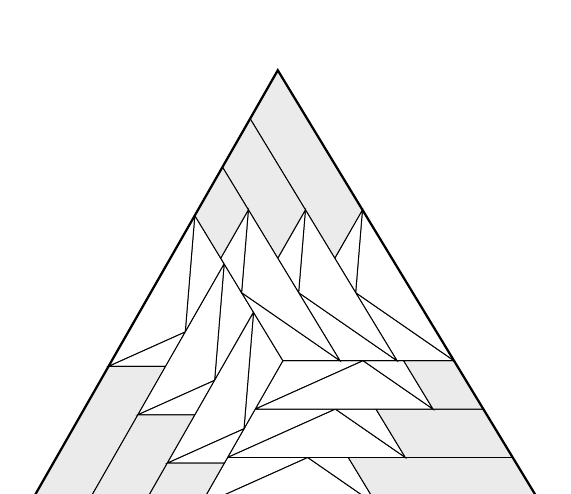
\begin{tikzpicture}[x={(0.0005cm,0cm)},y={(0.00025cm,0.0004330127019cm)},line width=0.35pt]
\draw[fill=white] (4320,0) -- (6345,1440) -- (4320,1440) -- cycle;
\draw[fill=white] (4320,0) -- (8809,0) -- (6345,1440) -- cycle;
\draw[fill=white] (6345,1440) -- (8809,0) -- (7369,1440) -- cycle;
\draw[fill=black!8] (8809,0) -- (12960,0) -- (11520,1440) -- (7369,1440) -- cycle;
\draw[fill=white] (4320,1440) -- (6345,2880) -- (4320,2880) -- cycle;
\draw[fill=white] (4320,1440) -- (8809,1440) -- (6345,2880) -- cycle;
\draw[fill=white] (6345,2880) -- (8809,1440) -- (7369,2880) -- cycle;
\draw[fill=black!8] (8809,1440) -- (11520,1440) -- (10080,2880) -- (7369,2880) -- cycle;
\draw[fill=white] (4320,2880) -- (6345,4320) -- (4320,4320) -- cycle;
\draw[fill=white] (4320,2880) -- (8809,2880) -- (6345,4320) -- cycle;
\draw[fill=white] (6345,4320) -- (8809,2880) -- (7369,4320) -- cycle;
\draw[fill=black!8] (8809,2880) -- (10080,2880) -- (8640,4320) -- (7369,4320) -- cycle;
\draw[fill=white] (0,8640) -- (1440,5175) -- (1440,7200) -- cycle;
\draw[fill=white] (0,8640) -- (0,4151) -- (1440,5175) -- cycle;
\draw[fill=white] (1440,5175) -- (0,4151) -- (1440,4151) -- cycle;
\draw[fill=black!8] (0,4151) -- (0,0) -- (1440,0) -- (1440,4151) -- cycle;
\draw[fill=white] (1440,7200) -- (2880,3735) -- (2880,5760) -- cycle;
\draw[fill=white] (1440,7200) -- (1440,2711) -- (2880,3735) -- cycle;
\draw[fill=white] (2880,3735) -- (1440,2711) -- (2880,2711) -- cycle;
\draw[fill=black!8] (1440,2711) -- (1440,0) -- (2880,0) -- (2880,2711) -- cycle;
\draw[fill=white] (2880,5760) -- (4320,2295) -- (4320,4320) -- cycle;
\draw[fill=white] (2880,5760) -- (2880,1271) -- (4320,2295) -- cycle;
\draw[fill=white] (4320,2295) -- (2880,1271) -- (4320,1271) -- cycle;
\draw[fill=black!8] (2880,1271) -- (2880,0) -- (4320,0) -- (4320,1271) -- cycle;
\draw[fill=white] (8640,4320) -- (5175,6345) -- (7200,4320) -- cycle;
\draw[fill=white] (8640,4320) -- (4151,8809) -- (5175,6345) -- cycle;
\draw[fill=white] (5175,6345) -- (4151,8809) -- (4151,7369) -- cycle;
\draw[fill=black!8] (4151,8809) -- (0,12960) -- (0,11520) -- (4151,7369) -- cycle;
\draw[fill=white] (7200,4320) -- (3735,6345) -- (5760,4320) -- cycle;
\draw[fill=white] (7200,4320) -- (2711,8809) -- (3735,6345) -- cycle;
\draw[fill=white] (3735,6345) -- (2711,8809) -- (2711,7369) -- cycle;
\draw[fill=black!8] (2711,8809) -- (0,11520) -- (0,10080) -- (2711,7369) -- cycle;
\draw[fill=white] (5760,4320) -- (2295,6345) -- (4320,4320) -- cycle;
\draw[fill=white] (5760,4320) -- (1271,8809) -- (2295,6345) -- cycle;
\draw[fill=white] (2295,6345) -- (1271,8809) -- (1271,7369) -- cycle;
\draw[fill=black!8] (1271,8809) -- (0,10080) -- (0,8640) -- (1271,7369) -- cycle;
\draw[line width=0.8pt] (0,0) -- (12960,0) -- (0,12960) -- cycle;
\end{tikzpicture}

\caption{The 36 macroregions of the exact construction. Shaded regions are strip parallelograms; the other regions are integer-scale copies of the tile. This shows the macro partition, not all 116640 individual triangles.}
\end{figure}

\subsection*{Coordinate details}
The basic $120^\circ$ trapezoid has
\[
 A=(0,0),\ B=(K+L,0),\ C=(K,L),\ D=(0,L),\ E=(a^2,L).
\]
The triangles $AED,ABE,EBC$ have scales $a,c,b$. In a band with shorter base $x$, the remainder is the parallelogram
\[
B,\ (x+L,0),\ (x,L),\ C.
\]
For the $60^\circ$ basic trapezoid take instead $E=(a^2,0)$ and triangles $AED,DEC,EBC$. Rotations by $120^\circ$ act as $(x,y)\mapsto(-x-y,x)$. Every macroregion coordinate in the supplied example is integral in this basis; small-tile coordinates are rational.

\section{Verification and remaining obligations}
The separate checker does not import the construction program. It checks every macroregion, all pair intersections by exact rational convex clipping, and equality of the covered area. Within each region, coverage and disjointness follow from the explicit standard quadratic triangle grids or strip-cell partitions.

\begin{center}
\begin{tabular}{lr}
\toprule
Retained exact check & Result\\
\midrule
Macroregions &36\\
Macroregion pairs checked &630\\
Positive-area macro overlaps &0\\
Expanded congruent triangles checked &116640\\
Supplementary primitive triples, $A\le250$ &102\\
Supplementary equilateral scale tests &4887\\
Supplementary ratio-family scale tests &8948\\
Supplementary macro constructions &52\\
Supplementary macro pair tests &51996\\
Altered certificates rejected &7\\
\bottomrule
\end{tabular}
\end{center}
All small triangles were explicitly checked for their three squared side lengths, area, and containment in their block and target. We did not perform the $O(N^2)$ pairwise small-triangle test: its disjointness claim rests on the stated standard subdivisions plus the checked macro partition. The expanded exact coordinates are supplied in a compressed JSON-lines file.

For each fixed tile, Theorems~\ref{thm:equilateral} and~\ref{thm:construction} leave only a finite interval of potentially exceptional small multipliers. The primitive tile parameters are unbounded, and other angular families also remain. A finite exception interval for each tile is not a finite global exception list. A necessary and sufficient classification for all $N$ in Erd\H{o}s problem 634 has not been obtained here.

\begin{thebibliography}{9}
\bibitem{Zhang} Yan X Zhang, \emph{Tiling Triangles with $2\pi/3$ Angles}, arXiv:2512.22696v4, 4 April 2026; manuscript dated 7 April 2026. \url{https://arxiv.org/abs/2512.22696v4}.
\bibitem{Bonfioli} Vico Bonfioli, \emph{A signed-direction invariant for triangle tilings, and the exclusion of primes congruent to 3 modulo 4}, source manuscript in \texttt{ElVec1o/erdos\_634\_proof}, inspected 30 September 2026. Specific input: the direction-functional framework and theorem labelled \texttt{thm:spectrum}; broader conditional prime claims are not inputs. Content blob SHA: \texttt{b7a471881297a7cb0e44dc80ae3f65df60e8e076}. \url{https://github.com/ElVec1o/erdos_634_proof/blob/main/paper/erdos-634.tex}.
\bibitem{Rationality} Michael Beeson and Yan X Zhang, \emph{Rationality of certain triangle tilings}, arXiv:2604.01314v1, Theorem 1.2. \url{https://arxiv.org/abs/2604.01314v1}.
\end{thebibliography}
\end{document}
